\chapter{Introducción}
\label{cap:capitulo1}
\setcounter{page}{1}

\begin{flushright}
\begin{minipage}[]{10cm}
\emph{Quizás algún fragmento de libro inspirador...}\\
\end{minipage}\\

Autor, \textit{Título}\\
\end{flushright}

\vspace{1cm}

El desarrollo tecnológico ha provocado el avance en la robótica, un campo muy amplio en la actualidad que está facilitando la vida a los humanos en distintos ámbitos, entre ellos, unos de los más importantes: la visión artificial,  cuyo objetivo es que los ordenadores sean capaces de percibir y entender el entorno, pudiendo así actuar por ellos mismos en función de la situación que se encuentren. \\
Para que la visión funcione correctamente, es necesario tener algoritmos de Deep Learning, que es la tecnología que permite a un ordenador aprender como un ser humano a base de entrenamiento. Esto tiene un gran impacto sobre el ser humano, ya que trabajos en los que se requiere la vigilancia o atención completa de una persona, podrían ser sustituidos por sistemas con visión artificial y Deep Learning.

\section{La robótica}
\label{sec:miseccion} % etiqueta para luego referenciar esta sección

La robótica, aunque no bajo ese nombre, se lleva utilizando desde hace mucho tiempo, siempre pensándola con el concepto de "herramientas automatizadas", desde Aristóteles hasta mediados del siglo pasado. Hasta entonces esta disciplina siempre se había entendido como máquinas que realizan un trabajo repetitivo por el ser humano, facilitándole a éste la vida. Esta concepción se refleja con Henry Ford y la producción en serie.\\
Sin embargo, la palabra \textit{robota} que significa "trabajo forzado", origen de la palabra robot, aparece por primera vez en 1921 en una obra de teatro de un autor checo llamado Karel Capek. Empezando a concebir esta palabra a principios de siglo pasado, empezó a nacer el desarrollo de la idea de robótica que tenemos hoy en día, en el que la concepción de robótica ya no es "herramienta automatizadas", sino una industria interdisciplinaria que surge de la intersección de la ciencia, la ingeniería y la tecnología, uniendo el conocimiento científico, computacional e informático, con diversas ramas de la ingeniería, ya que no solo implica el estudio de robots, sino de su diseño, programación y aplicación. Es un conjunto de múltiples disciplinas como la informática, la AI, la informática, la visión, la programación o el álgebra entre otras muchas.\\
Con el paso de estos últimos años la robótica ha adquirido un gran peso y un desarrollo convierte a las películas futuristas que surgían hace unos años en el presente y que, aunque queda todavía mucho camino por continuar en esta amplia disciplina, es, actualmente una realidad entre los humanos.\\

Esta disciplina tiene como fin ayudar al ser humano en todos los ámbitos, tanto en la vida cotidiana como en la vida profesional, evitando los trabajos peligrosos y aburridos, e incluso haciendo trabajos que el ser humano no sería capaz de hacer por si mismo en distintos sectores, como pueden ser la medicina, facilitando el trabajo a los científicos con  el robot Da Vinci  \ref{fig:robots}, uno de sus robots más famosos en el que recibiendo las órdenes que el cirujano comanda a través de la consola, es capaz de hacer cirugías de alta precisión, eliminando los tembleques que un humano pueda tener y aportando una mayor visión al cirujano; la robótica espacial, que permite que no sea necesaria la movilidad del humano además de portar sistemas sensoriales para las condiciones del entorno en otro planeta como el Curiosity  \ref{fig:robots}, cuya misión era evaluar la habitabilidad en Marte; frente a la radiación, pues es un trabajo que pondría en peligro a cualquier humano exponiéndole frente a la radioactividad del entorno, con el ejemplo de los robots que se usaron en Fukushima \ref{fig:robots} después que un tsunami y un terremoto provocasen el desastre, pudiendo acceder a la zona y poder limpiarla o en la industria del automóvil con los coches autónomos, donde es el propio coche capaz de realizar todas las funciones de conducción desde un punto A a un punto B sin necesidad de la intervención humana.
\begin{figure}[h!]
  \begin{center}
    \subfigure[Robot Da Vinci]{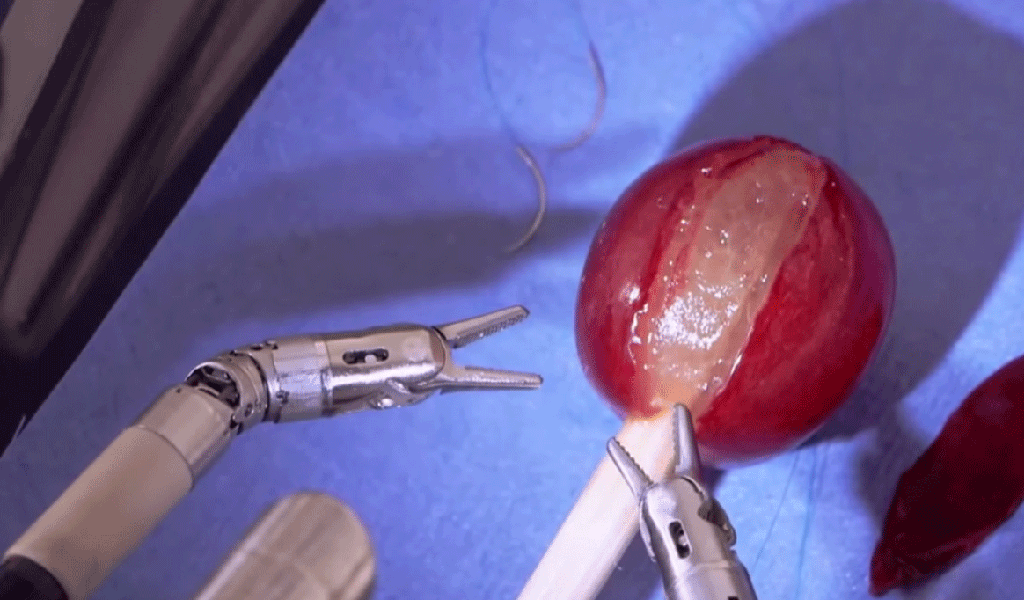
\includegraphics[width=45mm]{figs/da-vinci}}\hspace{8mm}
    \subfigure[Robot Curiosity]{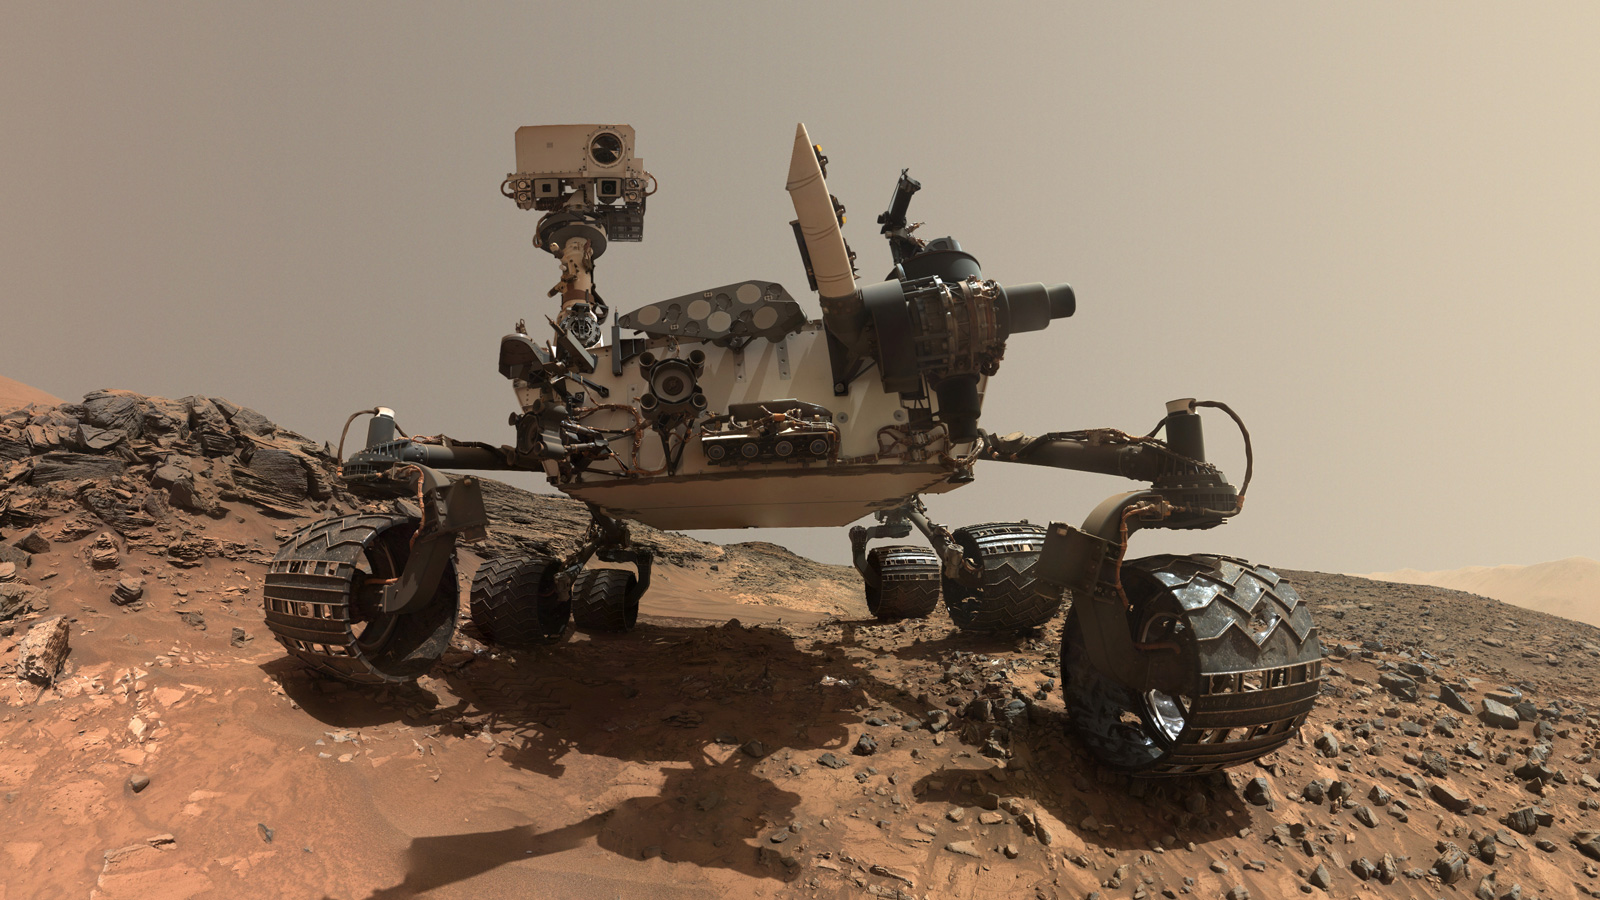
\includegraphics[width=48mm]{figs/curiosity}}\hspace{8mm}
    \subfigure[Uno de los robots de Fukushima]{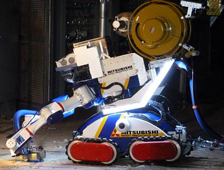
\includegraphics[width=40mm]{figs/fukushima}}
  \end{center}
\caption{Robots previamente mencionados.} \label{fig:robots}
\end{figure}

\subsection{Inteligencia Artificial}
La robótica es un conjunto de diferentes disciplinas que permiten abordar todos los campos que esta comprende. Uno de los campos en que a día de hoy la robótica está desarrollando y es muy importante es la AI, que consiste en replicar el funcionamiento mental a través del desarrollo de algoritmos para realizar determinadas tareas, e ir aprendiendo a medida que las realizan en base a la experiencia. Hay varios estudios en la actualidad con redes neuronales o algoritmos genéticos.\\
Hay dos tipos de inteligencia artificial:
\begin{itemize}
 \item{AI fuerte,} que está compuesta por la AI general, que es una teoría en la que una máquina tuviera una inteligencia humana, siendo capaz de resolver cualquier problema por sí misma; y la superinteligencia artificial, que superaría a la capacidad del cerebro humano. La AI fuete es todavía teórica y no hay ejemplos reales de su uso.
  \item{AI débil,} está entrenada para realizar tareas específicas, que operan dentro de un rango que previamente ha sido definido. Los sistemas dotados con esta inteligencia parecen inteligentes, pero están limitados y que no pueden realizar nada fuera de ese contexto, como es \textit{Siri de Apple}.
\end{itemize}\
La AI abarca diferentes campos como la comprensión, el reconocimiento y aprendizaje, \textit{a groso modo}, que a su vez, para su correcto funcionamiento, tienen extensos campos de estudio, entre los que destaca la visión artificial.\\

\subsection{Visión Artificial}
\label{sec:subseccion}
La visión artificial es uno de los campos más importantes de la AI que permite que los sistemas obtengan la información importante de imágenes digitales, vídeos u otras entradas visuales, y tomen acciones o hagan recomendaciones basadas en dicha información. Así pues, si la AI permite que los ordenadores piensen, la visión permite su observación, análisis y comprensión. Sin visión, una máquina no es capaz de reconocer ningún objeto, animal o persona en su entorno. \\
La visión artificial se trata de asemejar lo máximo posible a la visión humana, con la diferencia de que esta segunda cuenta con las experiencias aprendidas para diferenciar los elementos que le rodean, su movimiento, su distancia o su tamaño. Así pues la visión artificial trata de asemejar el funcionamiento del ojo humano y su posterior procesamiento con el cerebro con cámaras, datos y sensores para poder obtener la máxima información del entorno así como algoritmos para poder procesar la imagen adecuadamente, en el menor tiempo posible ya que es necesaria una reacción rápida.\\
Tiene diferentes usos, entre ellos los más fundamentales son:
\begin{itemize}
 \item \textit{Clasificación de imágenes \ref{fig:vision},}  que consiste en asignar imágenes en una serie de categorías predefinidas a través de un algoritmo. Es necesario contar con una gran cantidad de datos para poder tener suficiente entrenamiento para fallar lo mínimo posible.
 \item \textit{Detección de objetos \ref{fig:vision},} que consiste en analizar partes de la imagen para localizar objetos mediante cuadros limitadores. Esto se consigue mediante el entrenamiento de una gran cantidad de imágenes en las que se etiquetan diferentes tipos de objetos y etiquetándolos por su nombre, obteniendo así los datos que se usarán para la detección en una imagen.
  \item \textit{Segmentación de instancias \ref{fig:vision},} que consiste en el enmascaramiento exacto de los píxeles que representan a los objetos en una imagen. Es un paso más en la detección de objetos, siendo capaz de separar el objeto concreto del resto de la imagen. 
\end{itemize}\
\begin{figure}[h!]
  \begin{center}
    \subfigure[Clasificación de imágenes]{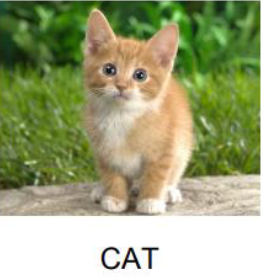
\includegraphics[width=43mm]{figs/clasificacion}}\hspace{8mm}
    \subfigure[Detección de objetos]{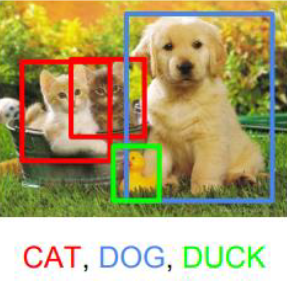
\includegraphics[width=45mm]{figs/deteccion}}\hspace{8mm}
    \subfigure[Segmentación de instancias]{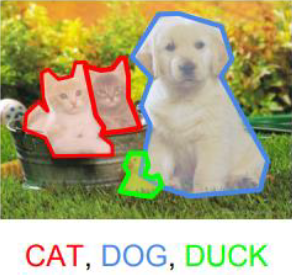
\includegraphics[width=47mm]{figs/segmentacion}}
  \end{center}
\caption[]{Algunos usos en la visión artificial.\footnotemark} \label{fig:vision}
\end{figure}\footnotetext{Imágenes obtenidas de shorturl.at/tyACR}\\
Un sistema dotado de visión funciona siguiendo tres niveles de operación:\\
En primer lugar, la obtención de imágenes o vídeos mediante una cámara. Estas imágenes son transferidas al sistema para poder procesarlas posteriormente. En segundo lugar, el procesamiento de las imágenes para poder representar correctamente los datos de interés. Este proceso consiste en un trabajo automático del sistema en el que se elimina el ruido, reescalar, ajustar el contraste y otros ajustes para adaptar las imágenes.\\ Finalmente, la comprensión de imágenes, que es el paso clave para que el sistema pueda llamarse inteligente, donde a través de un modelo de aprendizaje, es capaz de realizar el objetivo de interés, como puede ser detectar un determinado objeto utilizando datos aprendidos en el pasado.\\
Un ejemplo que está muy presente y en desarrollo actualmente es el caso de los coches autónomos \ref{fig:tesla}, que necesitan de una visión artificial impecable y sin fallos debido a que sus consecuencias pondrían en riesgo a los humanos. Estos coches utilizan distintos colores para detectar distintos elementos que puede encontrarse, como pueden ser líneas divisorias de la calzada, líneas delimitadoras de la calzada, semáforos, señales, objetos estáticos u objetos que se acercan. Así la computadora del coche procesa la información pudiendo detectar todo lo que afecta o potencialmente pueda afectar en la conducción y actúa en consecuencia.
\begin{figure} [h!]
  \begin{center}
    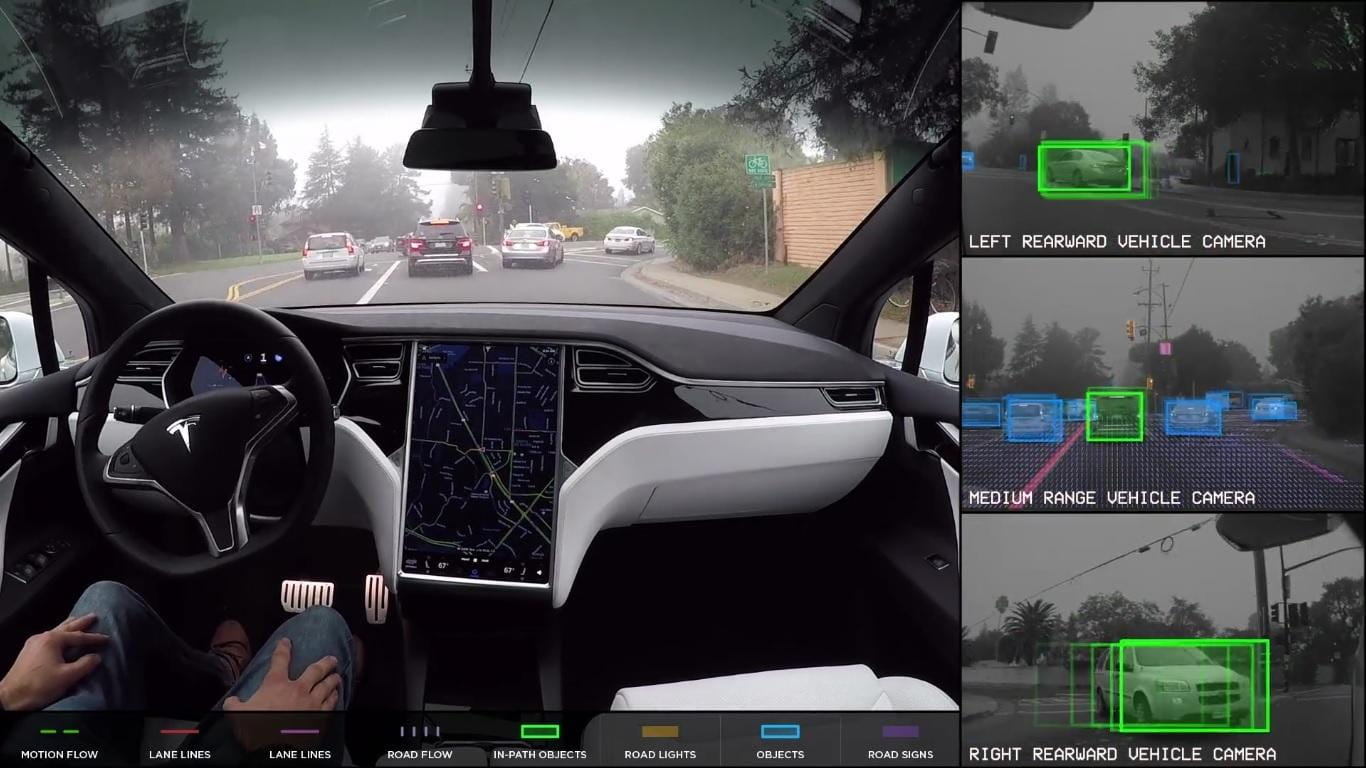
\includegraphics[width=8cm]{figs/coche_autonomo}
  \end{center}
  \caption[]{Vision de las cámaras y sensores de un Tesla autónomo. \footnotemark}
  \label{fig:tesla}
\end{figure}\footnotetext{Imágenes obtenidas de shorturl.at/huBFL}\\
Como se puede apreciar, es imprescindible disponer de una amplia cantidad de datos y de información basada en el aprendizaje pasado para que el algoritmo sea preciso y tenga el menor número de errores, para poder definirlo como robusto y fiable. Para lograr esto se pueden usar dos tecnologías; deep learning y una red neuronal convolucional o CNN.\\

\subsection{Machine Learning}
Es necesario dotar a los sistemas con una inteligencia artificial para poder conseguir que sean capaces de aprender automáticamente sin necesidad de ayuda externa. Dentro de la AI se encuentra una categoría denominada \textit{Machine Learning} o aprendizaje automático cuyo fin es que los algoritmos descubran patrones en conjuntos de datos que les hacen aprender y mejorar respecto a la experiencia anterior pudiendo así tener un aprendizaje autónomo para poder realizar una tarea sin ayuda externa.\\

En el sistema de aprendizaje de un algoritmo de \textit{Machine Learning} hay tres partes principales: En primer lugar un proceso de decisión, en el que una vez recibidos los datos de entrada, que pueden no estar etiquetados o bien estarlo para así indicarle al modelo lo que debe identificar, el algoritmo genera una estimación en los datos partiendo de un patrón.\\
La segunda parte es una función de error que sirve para evaluar la precisión del modelo sobre la decisión tomada, y la tercera y última parte es un proceso de optimización de modelos donde las ponderaciones se ajustan en el caso de que el modelo se pueda ajustar mejor a el conjunto de datos de entrenamiento, repitiendo este proceso hasta cumplir un umbral de precisión.

Hay diferentes tipos de \textit{Machine Learning}:
\begin{itemize}
 \item \textit{Aprendizaje supervisado,} en el que los conjuntos de datos para entrenar los datos que servirán como experiencia y base al algoritmo a la hora de hacer una clasificación con un nuevo dato están etiquetados, usando así un conjunto de datos entrenados iniciales a la hora de recibir un nuevo dato.
 \item \textit{Aprendizaje no supervisado,} en el que en este caso los datos están sin etiquetar, es decir, no cuenta con un conjuntos entrenado previamente.
 \item \textit{Aprendizaje semisupervisado,} que es el término medio entre los dos anteriores. En este caso, en el entrenamiento se usa un conjunto de datos más pequeño que en el aprendizaje supervisado y usa un grupo más grande de datos sin etiquetar.
\end{itemize}\

\subsection{Deep Learning}
Dentro del \textit{Machine Learning} se encuentra el \textit{Deep Learning} o aprendizaje profundo, que se diferencia del primero en el tipo de datos con el que trabaja así como en la manera en que aprende cada algoritmo, pues el \textit{Deep Learning} elimina algunos de los datos de preprocesado, eliminando gran parte de la intervención humana y aprendiendo autónomamente con cada nueva información que recibe y permitiendo conjuntos de datos más grandes.\\
El \textit{Deep Learning} es una forma especializada de \textit{Machine Learning}, capaz  de detectar las características de un conjunto de datos para clasificarlos en distintas clases y no necesitando a un humano para definir previamente estas características como sucedía con ML. A través de distintos procesos, el algoritmo se ajusta a la mayor exactitud, mejorando así la precisión para el próximo dato. Es la técnica que más se asemeja al aprendizaje humano, y lo hace usando redes neuronales, que tratan de asemejar el funcionamiento del cerebro con la combinación de distintos datos de entrada, pesos de ponderación y \textit{bias}. El \textit{Deep Learning} también puede ser de tipo supervisado o no supervisado, dependiendo de si los datos están o no etiquetados, como sucede en el \textit{Machine Learning}.\\
Las redes neuronales \ref{fig:red} consisten en distintas capas de nodos interconectados, donde cada nodo se basa en su capa anterior para refinar y optimizar la precisión. Está compuesto por la capas visibles, que son la primera, donde el modelo recibe los nuevos datos de entrada, y la última, donde se obtiene el resultado de predicción o clasificación, y las capaz ocultas o \textit{hidden layers} que son las que realizan todo el proceso de optimización hasta llegar al resultado final.\\
\begin{figure} [h!]
  \begin{center}
    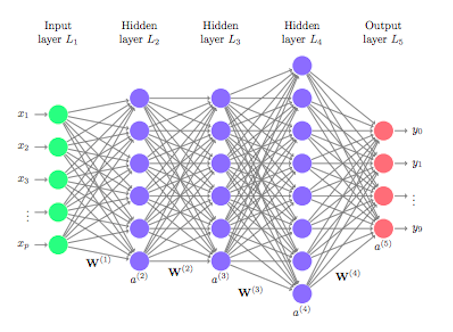
\includegraphics[width=8cm]{figs/deep_learning}
  \end{center}
  \caption[]{Simple ejemplo de una red neuronal en el algoritmo de Deep Learning. \footnotemark}
  \label{fig:red}
\end{figure}\footnotetext{Imágenes obtenidas de shorturl.at/kmpT5}\\

Este aprendizaje es una técnica muy importante a día de hoy que es necesaria para obtener resultados óptimos como en el campo de la visión artificial.\\
Algunas de las aplicaciones más conocidas o que acompañan a los humanos en su día a día son los coches autónomos, como se ha comentado anteriormente, que necesitan reconocer de manera inmediata qué decisiones tomar frente a la situación que se les presente, los asistentes virtuales, que son capaces de establecer una conversación, y que toman cada contacto con el usuario como un nuevo dato que utilizan para aprender continuamente, reconocimiento visual \ref{fig:visual} de caras, personas o elementos en imágenes o vídeos pudiendo detectar el objeto de interés, generación automática de texto o la traducción de este partiendo de imágenes, recomendaciones de películas o serie en base a los gustos de cada persona en plataformas como \textit{Netflix}, \textit{Spotify} o \textit{Amazon}, hasta en el campo de la biomedicina, siendo capaz de predecir los cambios en los procesos celulares debido a la variación genética o de detectar si las radiografías indican enfermedades, o con el Big Data, que son todos los datos básicos que se recogen constantemente de los humanos a través de internet donde el \textit{Deep Learning} es capaz de extraer análisis y aprender de todas estas cantidades de datos.
\begin{figure} [h!]
  \begin{center}
    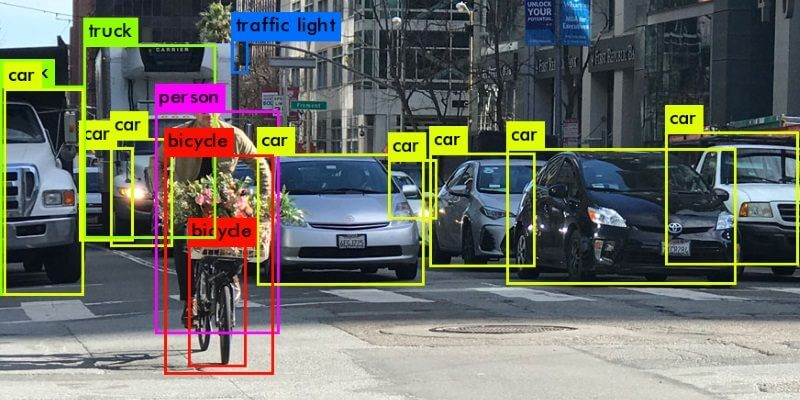
\includegraphics[width=8cm]{figs/visual_recognition}
  \end{center}
  \caption[]{Reconocimiento visual en visión con técnica de Deep Learning. \footnotemark}
  \label{fig:visual}
\end{figure}\footnotetext{Imágenes obtenidas de shorturl.at/kKRS6}\\

\subsection{Sistema multisensorial}
Debido a la importancia de las anteriores secciones y al auge que están teniendo en la actualidad, desde la robótica al \textit{Deep Learning}, la decisión de este trabajo ha sido realizar un sistema multisensorial monitorizado.\\
La base idea de este trabajo ha sido pensada para un laboratorio de animales, pues la robótica está presente en este ámbito así como en otros muchos aunque sin embargo, en este sector no trabajan ingenieros, por lo que puede haber trabajo que se realice en el laboratorio que podría mejorarse hasta incluso automatizarse. Para obtener más información, se ha contactado con el laboratorio de animales de la Universidad de Alcalá de Henares \footnote{\url{https://www.uah.es/es/}}  para conocer la situación en la que trabajan. Se ha notado que hay bastantes cosas que se podrían mejorar y se ha enfocado el objetivo en el estudio de los ratones del laboratorio, que requieren una observación constante así como del entorno en el que se encuentran debido a que que deben ser unas condiciones determinadas.\\
Después de conocer esta información la idea del trabajo ha tomado más forma e idea, decidiendo así componer un sistema multisensorial, que consiste en dotar a un computador de diferentes sensores que le permitan obtener datos del entorno que le rodea para poder actuar en función a ellos para ofrecer a la cubeta en la que se encuentran los ratones las mejores condiciones y así poder obtener parámetros importantes del entorno de los ratones como pueden ser la temperatura, humedad o calidad del aire. Así mismo, debido al desconocimiento de los trabajadores del laboratorio del mundo de la robótica y la ingeniería en general, se ofrece una interfaz gráfica donde los valores numéricos obtenidos por los sensores, así como cualquier interacción necesaria se traducen en \textit{widgets} comprensibles para cualquier usuario de una manera intuitiva y sencilla.\\
Por último, con una cámara, que es uno de los sensores incluidos en este sistema, se obtienen vídeos de los ratones, que, aplicando a la visión un algoritmo de \textit{Deep Learning} para realizar reconocimiento de objetos, en este caso, ratones, sea el sistema capaz de evaluar el tiempo que pasan los ratones en las diferentes zonas de la cubeta así como en cada una de las dos cubetas interconectadas por un tubo, evitando así el trabajo que tiene una persona a día de hoy de grabar vídeos de veinticuatro horas y visualizarlos para poder analizar las características del entorno y el comportamiento de los ratones sin automatización alguna.\\
Una característica extra a este sistema es que se ha realizado con una plataforma de bajo coste, lo que significa que tanto el sistema computacional como los sensores utilizados son económicamente accesibles para cualquier usuario, por lo que está al alcance de cualquier usuario que lo quiera incorporar.\\

\subsection{Comparación con otros sistemas del mercado}
Algunos de los sistemas que hay actualmente en el mercado son:
\begin{itemize}
 \item \textit{Sistema de monitorización en tiempo real la salud animal \footnote{\url{https://www.ucm.es/data/cont/docs/3-2017-05-22-2017_05_not5.pdf}}.} La Universidad Complutense de Madrid \footnote{\url{https://www.ucm.es}} realizó un sistema para detectar de forma temprana las enfermedades o infecciones que tienen síntomas febriles en animales de granja, más concretamente en cerdos. Este sistema se desarrolló con la instalación de microchips y otro tipo de sensores en los animales para poder controlar las condiciones como su temperatura o el consumo de agua de los bebederos, de forma que un ordenador muestra esta información de manera gráfica.\\
También se incluye una monitorización grupal mediante grabaciones diarias para que el sistema detecte cualquier tipo de actividad no común. 
\begin{figure} [h!]
  \begin{center}
    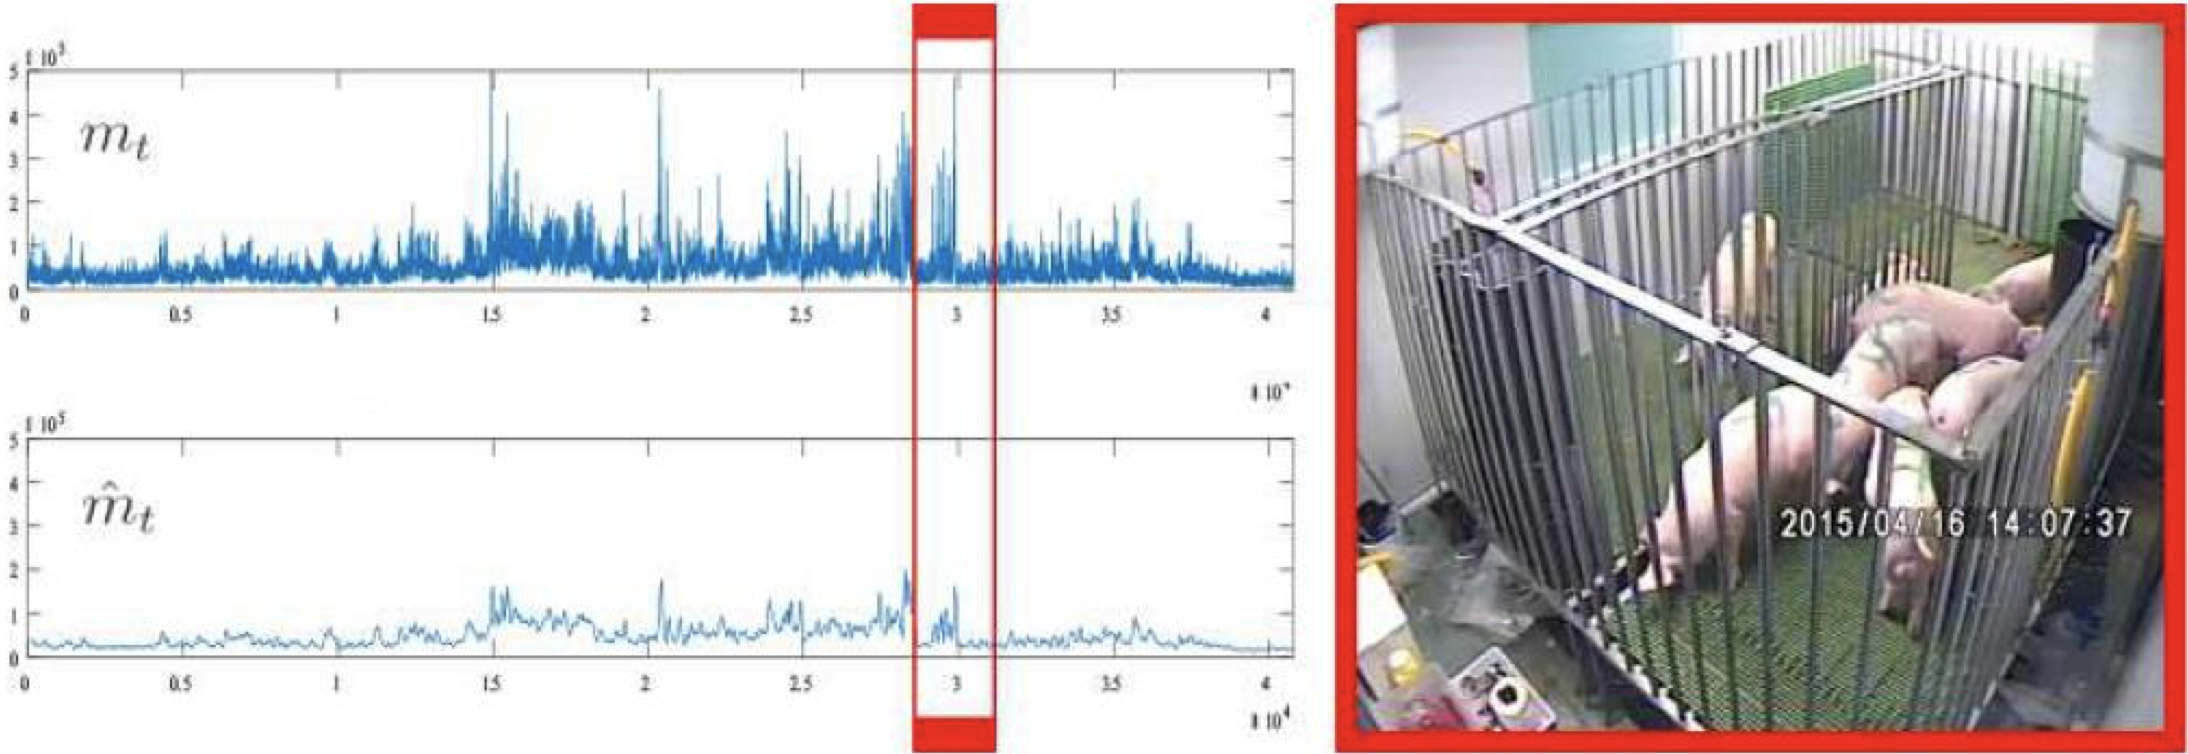
\includegraphics[width=10cm]{figs/ucm}
  \end{center}
  \caption{Patrón de movimientos e imagen grabada del grupo de cerdos.}
  \label{fig:uc}
\end{figure}\

\item \textit{Monitorización de rebaños de bovinos a través de redes de sensores inalámbricos \footnote{\url{https://scielo.isciii.es/scielo.php?script=sci_arttext&pid=S0004-05922009000200010}}.} La Facultad de Zootecnia e Ingeniería de la Universidad de São Paulo \footnote{\url{http://www.usp.br}} desarrolló un sistema de sensores con el fin de obtener datos fisiológicos de los animales, en este caso vacas, y obtener las condiciones en las que los animales tienen menos perturbaciones en su comportamiento natural, pues las condiciones climatológicas en cada región pueden afectar de diferentes maneras con estrés, pérdidas productivas o incluso la muerte.\
Este sistema se creó con la instalación de sensores en cada una de las vacas creando una red de sensores que se comunican con una estación para obtener todos los datos del conjunto de animales.
\begin{figure} [h!]
  \begin{center}
    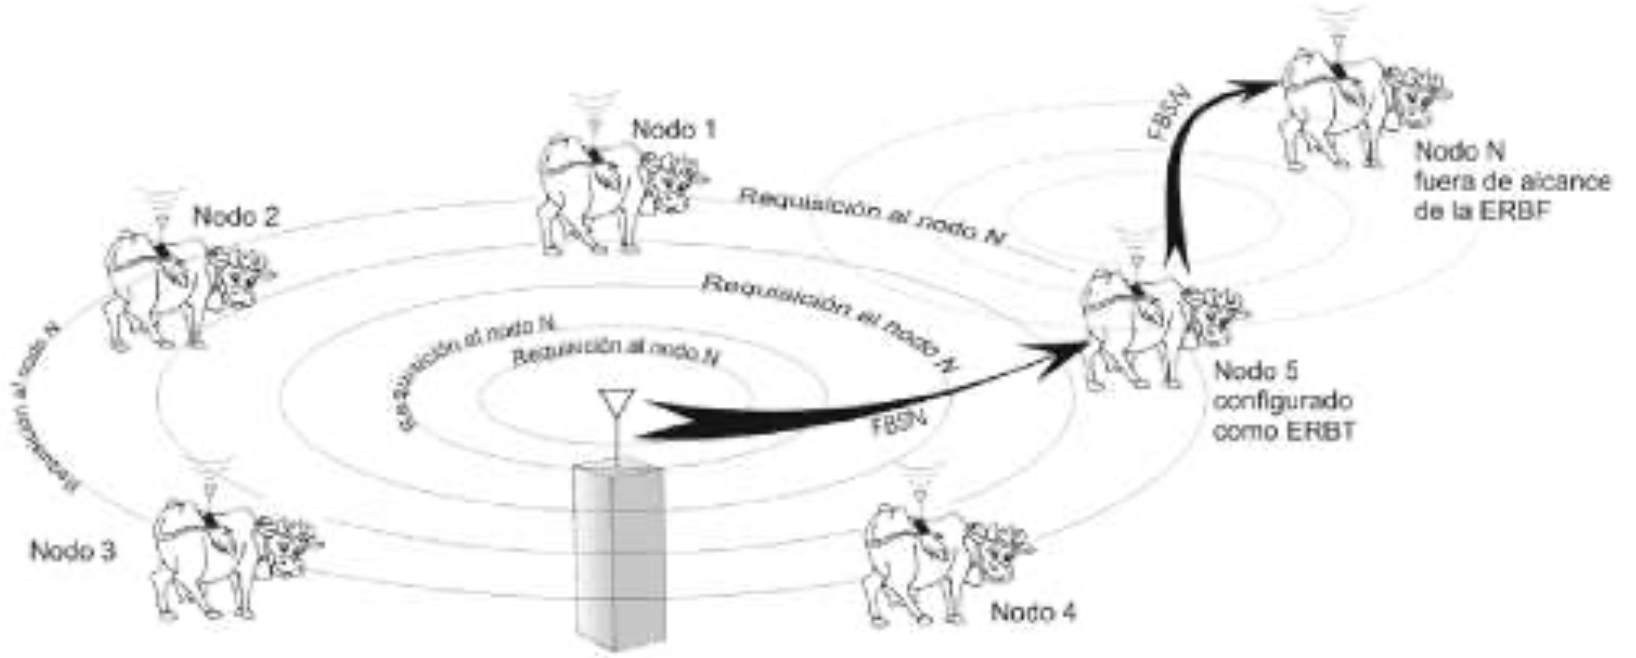
\includegraphics[width=10cm]{figs/saopaulo}
  \end{center}
  \caption{Esquema del desarrollo del sistema mediante sensores.}
  \label{fig:usao}
\end{figure}
\end{itemize}\

El comportamiento que tienen los animales puede ofrecer mucha información acerca de su salud si se mantiene una observación constante, pero también tienen una gran importancia las condiciones del entorno en la que se encuentran, ya que pueden ser decisivas para detectar el motivo de su comportamiento. Por ello, es importante tener un seguimiento constante y automatizado de estas características permitiendo al humano encargarse únicamente en controlar los datos que el sistema registra.

\

\

\

Y, para terminar este capítulo, resume brevemente qué vas a contar en los siguientes.
